\documentclass[11pt,openany]{book}
% #1-Asignatura
% #2-Curso
% #3-Nombre
% #4-Link
% #5-Foto

\newcommand{\portada}[5]{
    \begin{titlepage}
        \begin{center}
            \vspace*{0.5cm}
            
            % Titulo con #1 lo mas grande posible
            {\Huge \textbf{#1}}

            
            \vspace{0.5cm}
            \LARGE
            Curso #2 
            
            \vspace{1cm}
            
            \Huge{\textbf{Grupo Viterbi}}

            \vspace{1cm}
            
\includegraphics[width=0.6\textwidth]{assets/Img/UGR-Logo.png}
            
            \vspace{0.5cm}

            \huge
            PRÁCTICA 5- PROGRAMACIÓN DINÁMICA
            
            \Large
            \vspace{1cm}
            \textbf{Integrantes:}  \\ 
             % Array con los nombres de los integrantes y el correo
             \begin{center}
                \begin{tabular}{c c }
                    \textbf{Miguel Ángel De la Vega Rodríguez} & miguevrod@correo.ugr.es \\
                    \textbf{Alberto De la Vera Sánchez} & joaquinrojo724@correo.ugr.es \\
                    \textbf{Joaquín Avilés De la Fuente} & adelaveras01@correo.ugr.es \\
                    \textbf{Manuel Gomez Rubio} & e.manuelgmez@go.ugr.es \\
                    \textbf{Pablo Linari Perez} & e.pablolinari@go.ugr.es
                \end{tabular}
             \end{center}
            \vspace{0.8cm}
            
            
            \large
             \vspace{1cm}
            Facultad de Ciencias UGR\\
            Escuela Técnica Ingeniería Informática UGR\\
            Granada\\
            #2 
            
        \end{center}
    \end{titlepage}
}



\usepackage{assets/formulas}
\usepackage{float}
\hbadness=10000 % Suppress Underfull \hbox warnings

%========================================|Indice|===============================================%

\begin{document}
\portada{Algorítmica}{2023-2024}{Miguel Ángel De la Vega Rodríguez}{https://github.com/Miguevrgo/}{github.png}
\tableofcontents % Índice
\newpage %Salto de pagina tras el Indice


%======================================|Documento|==============================================%
\chapter{Autores}
\begin{itemize}
      \item \textbf{Miguel Ángel De la Vega Rodríguez:} 20\%
            \begin{itemize}
                  \item Plantilla y estructura del documento \LaTeX
                  \item Programación Viajante
                  \item Programación SumaMax (DyV)
                  \item Tests de eficiencia
            \end{itemize}
      \item \textbf{Joaquín Avilés De la Fuente:} 20\%
            \begin{itemize}
                  \item Programacion SumaMax (DyV)
                  \item Programación Viajante (DyV)
                  \item Estudio eficiencia teórica algoritmos específicos y DyV
                  \item Tests de eficiencia
            \end{itemize}
      \item \textbf{Alberto De la Vera Sánchez: } 20\%
            \begin{itemize}
                  \item Redacción \LaTeX
                  \item Estudio de umbrales teóricos y empíricos de DyV
                  \item Graficas y ajustes
            \end{itemize}
      \item \textbf{Manuel Gomez Rubio} 20\%
            \begin{itemize}
                  \item Programacion SumaMax (Kadane)
                  \item Programacion Losetas 
            \end{itemize}
      \item \textbf{Pablo Linari Pérez:} 20\%
            \begin{itemize}
                  \item Programacion SumaMax (Kadane)
                  \item Programacion Losetas 
            \end{itemize}
\end{itemize}

\chapter{Equipo de trabajo}

\begin{itemize}
    \item \textbf{Miguel Ángel De la Vega Rodríguez:} (Ordenador donde se ha realizado el computo)
          \begin{itemize}
              \item AMD Ryzen 7 2700X 8-Core
              \item 16 GB RAM DDR4 3200 MHz
              \item NVIDIA GeForce GTX 1660 Ti
              \item 1 TB SSD NvMe
          \end{itemize}
\end{itemize}

\chapter{Objetivos}
En esta práctica, se pretende resolver problemas de forma eficiente aplicando la técnica de
Divide y Vencerás. Para ello, se han planteado varios problemas cuya solución es conocida
(excepto para el problema del viajante), y se han implementado algoritmos que los resuelven
mediante el método convencional y mediante la técnica de Divide y Vencerás. Posteriormente, se ha buscado
un umbral en el cual ambos tengan el mismo tiempo de ejecución, finalmente, se ha buscado el
umbral óptimo para cada problema.
\chapter{Definicion Problema}
Para esta práctica se han planteado tres problemas diferentes, cada uno de ellos con una solución conocida
y que se ha implementado mediante la técnica de Divide y Vencerás. Los problemas planteados son los siguientes:
\section{Problema 1: Subsecuencia de suma máxima}
Dado un vector de enteros, se pide encontrar la subsecuencia de suma máxima, es decir, secuancia de elementos consecutivos
tanto positivos como negativos cuya suma sea la suma máxima posible. Para ello, se han implementado dos algoritmos, uno
que resuelve el problema mediante la técnica de Divide y Vencerás y otro que lo resuelve mediante el algoritmo de Kadane.
\section{Problema 2: Enlosar un espacio}
Dado un espacio de tamaño $n \times n$ (tomaremos una habitación cuadrada), donde $n=2^k \text{para algún } k \geq 1$ y un conjunto de losas en forma de \enquote{ele} , se pide encontrar la forma de enlosar
dicho espacio con este tipo de losas teniendo en cuanta que debemos dejar un espacio de$2 \times 2$ tamaño $1 \times 1$ sin enlosar que será lo
que llamaremos en este problema un sumidero. \\
La posición del sumidero será proporcionada por el problema indicada así por la celda $A[i][j] \text{ tq } 0 \leq i,j \leq n-1$ de 
nuestra matriz. Para cada baldosa que coloquemos en la matriz le asociaremos un identificador (entero) distinto.
\section{Problema 3: Viajante de comercio}
Dado un conjunto de puntos en un plano, se pide encontrar el camino más corto que pase por todos los puntos y vuelva al punto de partida. 
La representación de este problema viene dada por un viajante que necesita recorrer una serie de ciudades marcadas con puntos en un mapa y debemos
indicar el camino más corto para recorrerlos todos y volver a su casa. \\
Para calcular la distancia entre dos puntos usaremos la distancia euclídea, es decir,
dados los puntos $(x_1,y_1)$ y $(x_2,y_2)$ la distancia entre ellos será
\begin{equation*}
      dist((x_1,y_1), (x_2, y_2))=\sqrt{(x_1-x_2)^2+(y_1-y_2)^2}
\end{equation*}

Para ello, se han implementado dos algoritmos, uno que resuelve el problema
mediante la técnica de Divide y Vencerás, que divide el problema en subproblemas más pequeños y los resuelve de forma recursiva, y otro 
algoritmo de fuerza bruta que resuelve el problema de forma exacta, que como veremos más adelante en este documento no puede superar la cantidad de 12 puntos, pues
al tener una eficiencia de $O(n!)$, para $n>12$ el tiempo de ejecución es inviable. \\ \\

Para la mediciónde tiempos de ejecución, se han usado los siguientes tamaños de problema:
\begin{itemize}
      \item \textbf{Problema 1:} Tamaños de problema de 25000 a 5000000 con saltos de 25000
      \item \textbf{Problema 2:} Tamaños de problema de 4 a 10
      \item \textbf{Problema 3:} Tamaños de problema de 50 a 30000 con saltos de 1000. Destacar que hemos hecho otros tests con tamaños de problema mayores,
            pero usando archivos de tipo texto donde se identifican ciudades de un país y sus coordenadas.
\end{itemize}

\chapter{Algoritmo Especifico}
En este apartado, estudiaremos la eficiencia teórica, empírica e híbrida de los algoritmos especificos
de cada uno de los problemas.
\section{Problema 1: Subsecuencia de suma máxima.}
Para el primer problema, el algoritmo específico que empleamos es el algoritmo de Kadene.
\subsection{Estudio teórico}
\begin{lstlisting}
      int kadane(int *a, int size){
            int max_global = a[0];
            int max_current = a[0];

            for (int i = 1; i < size; i++) {
                  max_current = max(a[i], max_current + a[i]);
                  if (max_current > max_global) {
                        max_global = max_current;
                  }
            }
            return max_global;
      }
\end{lstlisting}
Como podemos observar la eficiencia del codigo en las líneas 6-8, tienen eficiencia O(1). Por tanto,
su tiempo de ejecución es constante y notaremos por a. Luego, el bucle for se ejecutará  $(size-1)-i+1 $
veces, es decir, $size-i$ veces. Sabiendo que el resto de líneas del código tienen eficienciaa O(1), tenemos
el siguiente resultado
\begin{equation*}
      \sum_{i=inicial}^{size-1} a
\end{equation*}
Tomaremos $size =  n$ e $inicial = 1$ para simplificar el cálculo y veamos que obtenemos ahora
\begin{equation*}
      \sum_{i=1}^{n-1} a = a \cdot \sum_{i=1}^{n-1} 1= a \cdot (n-1)
\end{equation*}
Es claro que $a \cdot (n-1) \in O(n)$ y por tanto la eficiencia teórica del algoritmo de kadane es $O(n)$.
\subsection{Estudio empírico}
\begin{center}
      \begin{figure}[H]
                  \centering
                  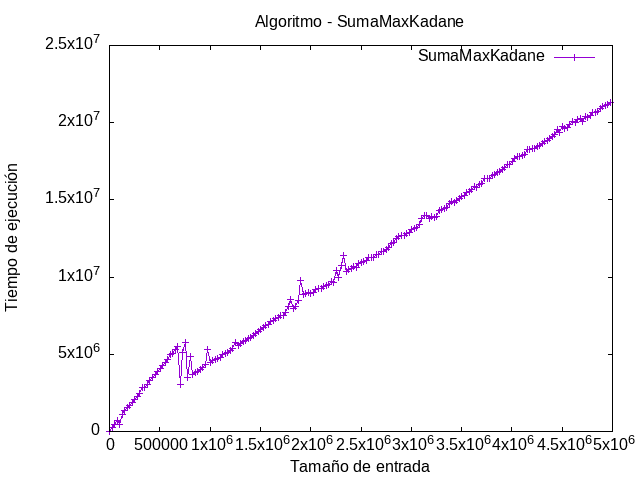
\includegraphics[width=0.7\linewidth]{assets/Img/SumaMaxKadane.png}
                  \caption{Ejecución algoritmo SumaMaxKadane}
                  \label{fig:SumaMaxKadane}
      \end{figure}
\end{center}
\subsection{Estudio híbrido}
\begin{center}
      \begin{figure}[H]
                  \centering
                  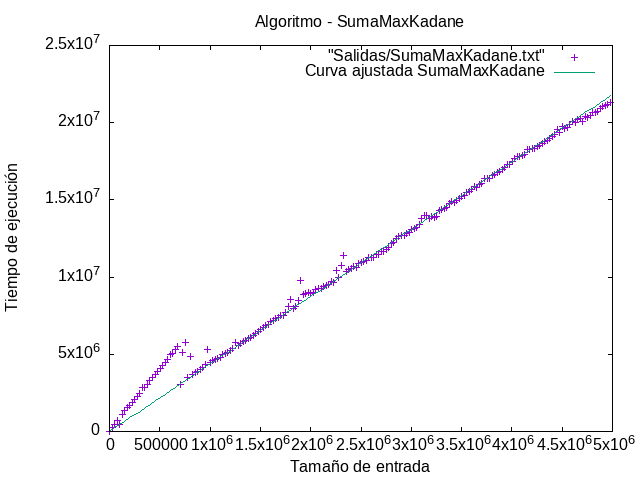
\includegraphics[width=0.7\linewidth]{assets/Img/SumaMaxKadane_hib.png}
                  \caption{Ajuste hibrido}
                  \label{fig:SumaMaxKadanehibrido}
      \end{figure}
\end{center}
Tras la interpretación de los datos empíricos en gnuplot y de la formula teorica del método, obtenemos que \\
las constantes ocultas son:
\begin{equation*}
      T_{Kadane}=1.64263x + 0.996451
\end{equation*}
\section{Problema 2: Enlosar un espacio }
Para el segundo problema el algoritmo específico que empleamos para resolver el problema es el siguiente : 

\begin{lstlisting}

      void resuelve2(int i,int j,int n, vector<vector<int>> & mat){
        losas++;
        for(int l = 0; l< n; l++){
            for(int k = 0; k<n; k++){
                if(mat[i+l][j+k] == 0){
                    mat[i+l][j+k] = losas;
                }
            }
        }
    
}
\end{lstlisting}
El código consiste en rellenar las posiciones de una matriz 2x2 con un valor entero en las posiciones donde el valor sea 0.
Podemos observar que hay dos bucles for anidados los cuales son $O(n)$ y el interior del bucle más profundo es $O(1)$ por tanto la eficiencia 
de este código es de $O(n^2)$

\section{Problema 3: Viajante de comercio }
Para el tercer problema el algoritmo específico que empleamos para resolver el problema es el siguiente : 

\subsection{Estudio teórico}
\begin{lstlisting}

      vector<Point> bruteForceTSP(const std::vector<Point>& points) {
            std::vector<int> permutation(points.size());
      
            std::iota(permutation.begin(), permutation.end(), 0);
        
            double minDistance = std::numeric_limits<double>::max();
            std::vector<int> bestPermutation;
            do {
                double distance = 0;
                for (int i = 0; i < permutation.size() - 1; ++i) {
                    distance += points[permutation[i]].distanceTo(points[permutation[i + 1]]);
                }
        
                distance += points[permutation.back()].distanceTo(points[permutation.front()]);
                if (distance < minDistance) {
                    minDistance = distance;
                    bestPermutation = permutation;
                }
            } while (std::next_permutation(permutation.begin(), permutation.end()));
        
            std::vector<Point> bestPath;
        
            for (int index : bestPermutation) {
                bestPath.emplace_back(points[index]);
            }
        
            return bestPath;
        }
\end{lstlisting}
Destacar que hemos implementado una clase Point que no tiene nada en particular, pues solo se ha implementado
como método útil el método \textbf{distanceTo(const \&Point p)} que calcula la distnacia entre dos puntos
mediante la distnacia euclídea, veámoslo:
\begin{lstlisting}
      double distanceTo(const Point &p) const {
            return sqrt(pow(x - p.x, 2) + pow(y - p.y, 2));
        }
\end{lstlisting}
Para estudiar la eficiencia de dicho algoritmo hay que tener claro como funcionan ciertas funciones de las librerías de C++, así como
su eficiencia teórica. En este caso, la función \textbf{std::iota} tiene eficiencia $O(n)$ y se encarga de rellenar un \textbf{vector<int>}
con una permutación que se inicia en $0$ (último parámetro dado) y acaba en $n-1$ (tamaño del vector), definido a partir de los puntero al inicio
y final del vector. \\
Por otro lado, la función \textbf{std::next\_permutation} tiene eficiencia $O(n)$ y se encarga de generar la siguiente permutación posible, devolviendo
 false si ya ha devuelto todas las permutaciones posible. Por tanto, el bucle do-while se ejecutará $n!$ veces, donde $n$ es el tamaño del vector de puntos. \\ \\

Por ahora tenemos una eficiencia de $O(n)$ en la llamda a la función \textbf{std::iota}, el bucle \textbf{do-while}, que acontinuación veremos su eficiencia, y el 
bucle for de la línea 24 que es claro que tiene eficiencia $O(n)$ pues recorre la mejor permutación con $n$ elementos, es decir, tenemos que la eficiencia teórica
de dicha función es $max\{O(\text{bucle do-while}), O(n)\}$. \\
Dentro del bucle \textbf{do-while} tenemos un bucle for que recorre la permutación de tamaño $n$ y realiza una operación de eficiencia $O(1)$, por tanto, la eficiencia
del bucle for es $O(n)$. El resto de operaciones de dicho bucle son de eficiencia $O(1)$, por lo que la eficiencia del bucle \textbf{do-while} es $O(n\cdot n!)$, es decir,
la eficiencia de la función es $O(n\cdot n!)$.
\subsection{Estudio empírico}
En esta parte el estudio empírico lo hemos realizado hasta el valor n=13 ya que sino el tiempo de ejecución pasaba a ser excesivo
\begin{center}
      \begin{figure}[H]
                  \centering
                  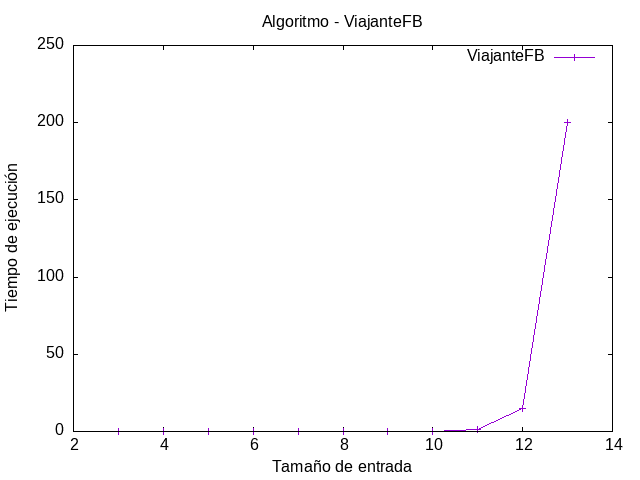
\includegraphics[width=0.7\linewidth]{assets/Img/ViajanteFB.png}
                  \caption{Ejecución algoritmo viajante fuerza bruta}
                  \label{fig:ViajanteFB}
      \end{figure}
\end{center}
\subsection{Estudio híbrido}
\begin{center}
      \begin{figure}[H]
                  \centering
                  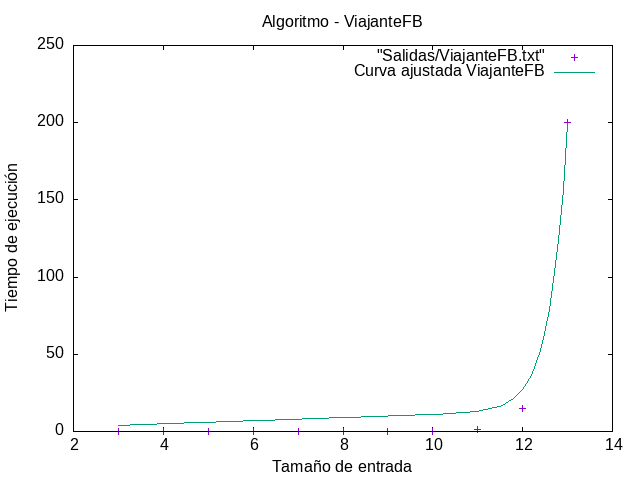
\includegraphics[width=0.7\linewidth]{assets/Img/ViajanteFB_hib.png}
                  \caption{Ajuste hibrido}
                  \label{fig:ViajanteFBhibrido}
      \end{figure}
\end{center}
Tras la interpretación de los datos empíricos en gnuplot y de la formula teorica del métoco, obtenemos que \\
las constantes ocultas son:
\begin{equation*}
      T_{ViajanteFB}=2.97582 \cdot 10^{-8}x!+x+1
\end{equation*}



\chapter{Algoritmo Divide y Vencerás}
En este apartado, estudiaremos la eficiencia teórica, empírica e híbrida de los algoritmos divide y vencerás
de cada uno de los problemas.
\section{Problema 1: Subsecuencia de suma máxima.}
Para el primer problema, el algoritmo DyV que empleamos es el siguiente:
\subsection{Estudio teórico}
\begin{lstlisting}
      int maxSubArray(const int * const arr, int low, int high, int threshold) {
          if (high - low + 1 <= threshold) {
              return kadane(arr, low, high);
          }
      
          int mid = low + (high - low) / 2;
      
          int leftSum = maxSubArray(arr, low, mid, threshold);
          int rightSum = maxSubArray(arr, mid + 1, high, threshold);
      
          int crossLeftSum = numeric_limits<int>::min();
          int crossRightSum = numeric_limits<int>::min();
          int sum = 0;
      
          for (int i = mid; i >= low; --i) {
              sum += arr[i];
              crossLeftSum = max(crossLeftSum, sum);
          }
      
          sum = 0;
          for (int i = mid + 1; i <= high; ++i) {
              sum += arr[i];
              crossRightSum = max(crossRightSum, sum);
          }
      
          int crossSum = crossLeftSum + crossRightSum;
      
          return max(max(leftSum, rightSum), crossSum);
      }
\end{lstlisting}
Este algoritmo hace usa de la técnica de \textbf{Divide y Vencerás} para resolver el problema de la subsecuencia de suma máxima, en el cual se divide el 
problema en subproblemas más pequeños y se resuelven de forma recursiva. Como se observa se usa el \textbf{algoritmo de Kadane} para resolver el caso base dado como el parámetro
\textbf{threshold}.\\ \\
El caso base solo usará cuando lleguemos a tamaños del problema menores o iguales a \textbf{threshold}, por lo que podemos obviar su eficiencia, ya que tardará
un tiempo constante en resolverlo. Por otro lado, el resto de las operaciones son la mayoría de eficiencia $O(1)$, excepto los bucles for que tienen eficiencia $O(n/2)=O(n)$ y las llamadas
recursivas al algoritmo con un tamaño $n/2$ (destacar que tomaremos $n=high-low$ como el tamaño del problema). Tomando estas ideas previas y usando la regla
del máximo, veamos los calculos de la eficiencia teórica:

\begin{equation*}
      T(n)=2T(\frac{n}{2})+n
\end{equation*}
  Pasemos ahora a resolver dicha ecuación de recurrencia. Aplicando el siguiente cambio de variable $n=2^m$ obtenemos
\begin{equation*}
      T(2^m)=2T(2^{m-1})+2^m \Rightarrow T(2^m)-2T(2^{m-1})=2^m
\end{equation*}
  Resolvamos la parte homógenea de la ecuación, es decir, la ecuación $T(2^m)-2T(2^{m-1})=0$. Obtenemos el polinomio
  característico de la parte homógenea que es $p_H(x)=x-2$ cuya raíz es $x=2$. \\
  Obtengamos ahora la parte no homógenea
\begin{equation*}
      2^m=b_1^m q_1(m) \Rightarrow b_1=2 \wedge q_1(m)=1 \text{ con grado } d_1=0
\end{equation*}
  Tenemos entonces el siguiente polinómio característico
\begin{equation*}
      p(x)=(x-2)(x-b_1)^{d_1+1}=(x-2)^2
\end{equation*}
  Por tanto la solución general es
\begin{equation*}
      t_m=c_{10}2^mm^0+c_{11}2^mm^1  \overset{*}{\Rightarrow}  t_n=c_{10}n+c_{11}n\log_2(n) \Rightarrow T(n)=c_{10}n+c_{11}n\log_2(n)
\end{equation*}
  donde en ($*$) hemos deshecho el cambio de variable \\
  Aplicando la regla del máximo tenemos $T(n) \in O(n\log(n))$

\subsection{Estudio empírico}
\begin{center}
      \begin{figure}[h]
            \centering
            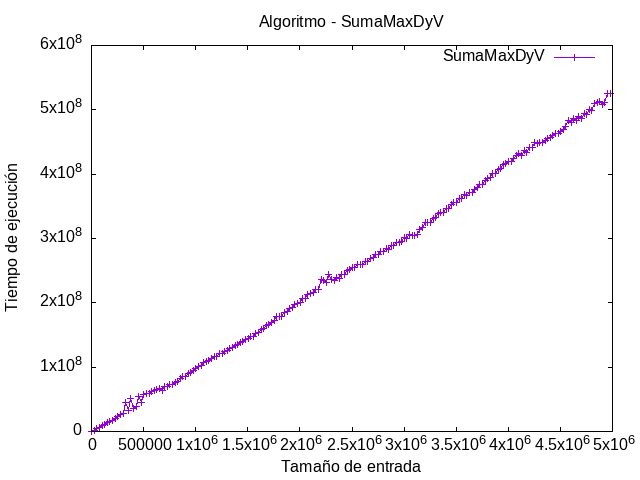
\includegraphics[width=0.7\linewidth]{assets/Img/SumaMaxDyV.png}
            \caption{Ejecución algoritmo SumaMaxDyV}
            \label{fig:SumaMaxDyV}
      \end{figure}
\end{center}
Como podemos observar en la gráfica, el algoritmo de DyV 
\newpage
\subsection{Estudio híbrido}
\begin{center}
      \begin{figure}[h]
            \centering
            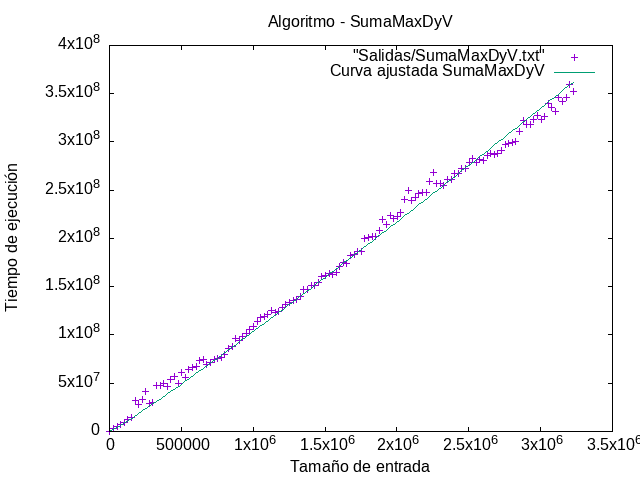
\includegraphics[width=0.7\linewidth]{assets/Img/SumaMaxDyV_hib.png}
            \caption{Ajuste híbrido algoritmo SumaMaxDyV}
            \label{fig:sumaMax}
      \end{figure}
\end{center}
Tras la interpretación de los datos empíricos en gnuplot y de la formula teorica del método, obtenemos que \\
las constantes ocultas son:
\begin{equation*}
      T_{SumaMaxDyV}=1.65508x + 0.991967
\end{equation*}
\subsection{Cálculo del umbral teórico}

\newpage
\section{Problema 2: Enlosar un espacio }
Para el segundo problema, el algoritmo DyV que empleamos es el siguiente:
\subsection{Estudio teórico}
\begin{lstlisting}
      void resolver(int n,int i,int j,vector<vector<int>> &mat){
            if(n == 2){
                  resuelve2(i, j, n, mat);
            }
            else{
                  getSumidero(i,j,mat,n);
                  if(i_sumidero < i + n/2  && j_sumidero < j + n/2){
                        enlosar(i+n/2-1,j+n/2,i+n/2,j+n/2-1,i+n/2,j+n/2,mat);
                  }
                  else if(i_sumidero >= i+n/2 && j_sumidero < j +n/2){ 
                        enlosar(i+n/2-1,j+n/2 -1, i+n/2 -1 , j+n/2 , i+n/2 ,j + n/2 ,mat);
                  }
                  else if(i_sumidero < i +n/2 && j_sumidero >= n/2 + j){ //Superior izquierda
                        enlosar(i+n/2-1,j+n/2 -1, i+n/2 , j+n/2-1 , i+n/2 ,j + n/2 ,mat);
                  }
                  else{
                        enlosar(i+n/2-1,j+n/2 -1, i+n/2 , j+n/2-1 , i+n/2 -1 ,j + n/2 ,mat);
                  }
                  resolver(n/2,i,j,mat);
                  resolver(n/2,i+n/2,j,mat);
                  resolver(n/2,i,j+n/2,mat);
                  resolver(n/2, i+n/2, j+n/2, mat);
            }


      }
\end{lstlisting}

Como el código se sustenta de la implementación de if/else anidados, su eficiencia teórica se calculará
sobre el bloque de sentencias dentro de un if/else con peor eficiencia. Además, vemos que intervienen 
dos llamadas a funciones dentro del segundo else.

\begin{lstlisting}
      void getSumidero(int i , int j , vector<vector<int>> & mat ,int n){
            for (int x = i; x< i + n; x++) {
                  for (int y = j; y < j + n; y++) {
                        if (mat[x][y] != 0)
                              i_sumidero = x, j_sumidero = y;
                  }   
            }
      }

      void enlosar(int i1, int j1,int i2 , int j2 , int i3 , int j3,vector<vector<int>> &mat){
            losas++;
            mat[i1][j1] = losas;
            mat[i2][j2] = losas;
            mat[i3][j3] = losas;

      }
\end{lstlisting}
De aquí, tenemos que la eficiencia de la función getSumidero es claramente $O(n^2)$. Mientras que la llamada
a función enlosar $O(1)$. A partir de esto, podemos calcular la eficiencia total del codigo resuelve:

\begin{gather*}
      T(n)= 4T(\frac{n}{2})+n^2
\end{gather*}
Pasemos ahora a resolver dicha ecuación de recurrencia. Aplicando el siguiente cambio de variable $n=2^m$ obtenemos
\begin{equation*}
      T(2^m)=4T(2^{m-1})+4^m \Rightarrow T(2^m)-4T(2^{m-1})=4^m
\end{equation*}
  Resolvamos la parte homógenea de la ecuación, es decir, la ecuación $T(2^m)-4T(2^{m-1})=0$. Obtenemos el polinomio
  característico de la parte homógenea que es $p_H(x)=x-4$ cuya raíz es $x=4$. \\
  Obtengamos ahora la parte no homógenea
\begin{equation*}
      4^m=b_1^m q_1(m) \Rightarrow b_1=4 \wedge q_1(m)=1 \text{ con grado } d_1=0
\end{equation*}
  Tenemos entonces el siguiente polinómio característico
\begin{equation*}
      p(x)=(x-4)(x-b_1)^{d_1+1}=(x-4)^2
\end{equation*}
  Por tanto la solución general es
\begin{equation*}
      t_m=c_{10}4^mm^0+c_{11}4^mm^1  {\Rightarrow}  t_m=c_{10}(2^{m})^2m^0+c_{11}(2^{m})^2m^1  
\end{equation*}
Deshacemos el cambio de variable
\begin{equation*}
      t_n=c_{10}n^2+c_{11}n^2\log_2(n) \Rightarrow T(n)=c_{10}n^2+c_{11}n^2\log_2(n)
\end{equation*}

  Aplicando la regla del máximo tenemos $T(n) \in O(n^2\log(n))$
\subsection{Estudio empírico}

A continuación  vemos la gráfica del algoritmo del problema 3 con una entrada de datos de matrices de dimensión $2^n$ con $2<=|n<=|17$ y con 
los sumideros colocados de forma aleatoria.
\begin{center}^
      \begin{figure}[H]
            \centering
            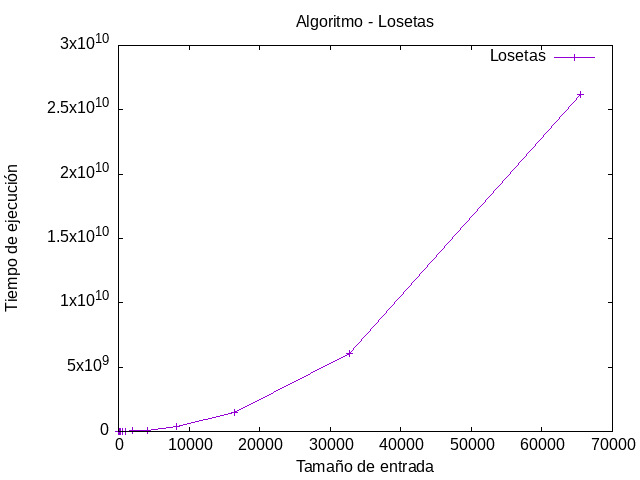
\includegraphics[width=0.7\linewidth]{assets/Img/Losetas.png}
            \caption{Ejecución algoritmo Losetas}
            \label{fig:Viajante}
      \end{figure}
\end{center}

\section{Problema 3: Problema del viajante de comercio.}
Para el tercer problema, nos encontramos ante un problema de complejidad
NP-duro, por lo que no podemos encontrar una solución exacta en tiempo polinómico.
Sin embargo, podemos encontrar una solución aproximada aplicando la técnica de Divide y Vencerás.
Para ello, usamos el algoritmo de fuerza bruta para encontrar la solución exacta para subconjuntos
del problema total y luego unimos las soluciones parciales para obtener una solución que se optimiza
para asegurar un cierto mínimo de precision.

\subsection{Estudio teórico}
Para el tercer problema, el algoritmo DyV que empleamos es el siguiente:
\begin{lstlisting}
      std::vector<Point> divideAndConquerTSP(const std::vector<Point>& points) {
            if (points.size() <= UMBRAL) {
                return bruteForceTSP(points);
            }
        
            int mid = points.size() / 2;
            std::vector<Point> left(points.begin(), points.begin() + mid);
            std::vector<Point> right(points.begin() + mid, points.end());
        
            std::vector<Point> leftTour = divideAndConquerTSP(left);
            std::vector<Point> rightTour = divideAndConquerTSP(right);
        
            std::vector<Point> combinedTour = leftTour;
            combinedTour.insert(combinedTour.end(), rightTour.begin(), rightTour.end());
        
        
            return optimizeTour(combinedTour);
        }

std::vector<Point> optimizeTour(const std::vector<Point>& tour) {
      std::vector<Point> currentTour = tour;
      bool improvement = true;

      while (improvement) {
            improvement = false;

            for (int i = 1; i < currentTour.size() - 2; ++i) {
                  for (int j = i + 2; j < currentTour.size(); ++j) {

                  double originalDistance = currentTour[i - 1].distanceTo(currentTour[i]) +
                                                currentTour[j - 1].distanceTo(currentTour[j]);
                  double swappedDistance = currentTour[i - 1].distanceTo(currentTour[j - 1]) +
                                          currentTour[i].distanceTo(currentTour[j]);

                  if (swappedDistance < originalDistance) {
                        std::reverse(currentTour.begin() + i, currentTour.begin() + j);
                        improvement = true;
                  }
                  }
            }
      }

      return currentTour;
}
\end{lstlisting}

En primer lugar, destacar que obviaremos el caso base, pues su eficiencia es constante y no afecta al cálculo de la eficiencia, por tanto, nos centraremos en el 
resto del algoritmo. \\
Como podemos observar, el algoritmo divide el problema en dos subproblemas de tamaño $n/2$ y los resuelve de forma recursiva. A continuación, se define un vector
de puntos que será la solución y para combinar los resultados simplemente uniremos las soluciones parciales, mediante el \textbf{.insert} de la STL de C++, lo cual
tiene una eficiencia $O(1)$ porque los insertamos al final.  \\ \\ 
En cuanto a la función \textbf{optimizeTour}, resulta claro que se ejecuta
$n-2$ veces el primer bucle y $n-1$ veces el segundo, estos nos da una eficiencia en el peor caso de 
$O(n^2)$, esta situación se da cuando en cada iteración del bucle, el cambio propuesto nos proporciona
una mejora, por lo que el bucle \textit{while} se ejecuta mientras lo hagan los bucles \textit{for}. Veamos ahora los calculos para la eficiencia teórica del algoritmo
implementado de DyV: 
\begin{equation*}
      T(n)=2T\left(\frac{n}{2}\right)+n^2
\end{equation*}

Pasemos ahora a resolver dicha ecuación de recurrencia. Aplicando el siguiente cambio de variable $n=2^m$ obtenemos
\begin{equation*}
      T(2^m)=2T(2^{m-1})+2^{2m} \Rightarrow T(2^m)-2T(2^{m-1})=2^{2m}
\end{equation*}
  Resolvamos la parte homógenea de la ecuación, es decir, la ecuación $T(2^m)-2T(2^{m-1})=0$. Obtenemos el polinomio
  característico de la parte homógenea que es $p_H(x)=x-2$ cuya raíz es $x=2$. \\
  Obtengamos ahora la parte no homógenea
\begin{equation*}
      2^{2m}=b_1^m q_1(m) \Rightarrow b_1=2^2=4 \wedge q_1(m)=1 \text{ con grado } d_1=0
\end{equation*}
  Tenemos entonces el siguiente polinómio característico
\begin{equation*}
      p(x)=(x-2)(x-b_1)^{d_1+1}=(x-2)(x-4)
\end{equation*}
  Por tanto la solución general es
\begin{equation*}
      t_m=c_{10}2^mm^0+c_{20}4^mm^0\overset{*}{\Rightarrow}  t_n=c_{10}n+c_{20}n^2 \Rightarrow T(n)=c_{10}n+c_{20}n^2
\end{equation*}
  donde en ($*$) hemos deshecho el cambio de variable \\
  Aplicando la regla del máximo tenemos $T(n) \in O(n^2)$

\subsection{Estudio Empírico}
Para determinar el umbral con el que obtenemos la mejor relación entre eficiencia y precisión, hemos
realizado una serie de pruebas con diferentes valores de umbral, a partir de tamaño 10, el algoritmo de
fuerza bruta se vuelve completamente inviable, de forma similar, para tamaño menor a 4, el algoritmo
no nos produce ninguna mejora en cuanto a eficiencia debido a la cantidad de llamadas recursivas que
saturan la pila, y la precision disminuye de forma considerable. Por ello, hemos decidido realizar
las pruebas para tamaños de 4 a 10, con distintas ciudades con solución ya conocida, para comparar
los tiempos de ejecución y la precisión de los resultados obtenidos:
\subsubsection*{Tiempo de ejecución}
\begin{center}
      \begin{figure}[H]
            \centering
            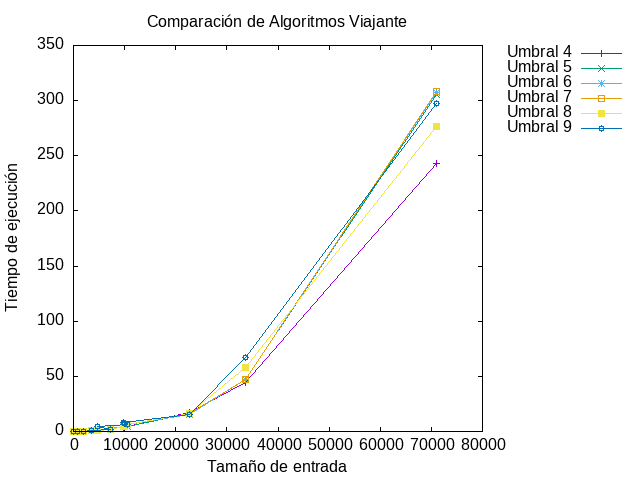
\includegraphics[width=0.7\linewidth]{assets/Img/UmbralP3.png}
            \caption{Ejecución algoritmo Viajante}
            \label{fig:Viajante}
      \end{figure}
\end{center}muchos
Como se puede apreciar, los mejores resultados se han obtenido con los umbrales $\{4,8\}$.
Para decididir cual de los dos umbrales es el mejor, nos fijamos en la precisión
que nos proporciona cada uno de ellos:
\subsubsection*{Precisión}



\chapter{Conclusiones}

Tras haber resuelto los problemas propuestos en la práctica hemos podido observar la eficacia
de usar una técnica como la de divide y vencerás la cual hace que de un problema aparentemente 
extenso y con una gran variedad de casos se pueda resolver dividiendolo  en subproblemas hasta llegar 
a un caso base (umbral) donde resolvamos el problema con un algoritmo sencillo como es el caso de 
el problema 2 en el cual el caso base es tan simple com rellenar una matriz 2x2 . En otros casos como 
el problema de la suma máxima o  el viajero  el algoritmo base es más complejo pero esto hace que se pueda ver la esencia del 
divide y vencerás que con saber resolver un caso base , los demás casos son solo una ampliación de este por tanto podemos conseguir una
eficiencia considerablemente buena con grandes cantidades de datos  aún usando algoritmos no tan eficientes con esa cantidad de  datos en el caso base.

También se ve reflejada la importancia de los umbrales los cuales pueden hacer que el problema sea mas o menos eficiente 
dependiendo de lo preciso que sea el umbral y la distinción entre casos que se hayan  hecho ya que una mala elección 
del umbral en el que se usa el algoritmo del caso base puede llevar a un gran lastre en la eficiencia de nuestro algoritmo 
ya que estaremos sometiendo al algoritmo  base a más datos de los necesarios para que sea eficiente .

\end{document}